\chapter{Software design and implementations for MLIP}

%\chapter{Implementations for MLIP for analysis of BaTiO_3}
%The technical barbone of the how this work contributed to application work as the analysis of interfacial effects $BaTiO_3$.

As scientific methods continue to evolve, the demands placed on software to incorporate these advancements also grow.
%While advances in methodolgy can prove to improve a method in all aspects, and thus replace an existing method, it is more often the case that they extend the capabilities and requiring more flexibility of the software outside of the initial design of the software package.
While improvements in method development often lead to enhanced efficiency and user-friendliness, they typically extend the software's capabilities beyond its original design.
As software is extended by more features over time, it tends to become less adaptable to changes to incorperate newly developed methods.
Consequently, rapid advancements in methodology can render software obsolete before the development is even at the stage of deployment for experiments.
%Considering that software becomes more rigid to changes over time with increased number of implemented features, it is a natural consequence that with a rapid development in methodology the software becomes deprecated as it cannot keep up with these changes.
Similar challenges were observed in the 1960s when rapid hardware development contributed to a software crisis\cite{brian2012software_crisis}.
However, as development progresses, also the understanding of critical components for performance emerges which solidifies the possible software designs to retrieve performant code.
With this places in the software naturally appear that can be used to decompose it into separate components allowing to distribute the software development workload among peers.
%groups as they can independently work on the individual modules.
This not only allows to speed up the development but it also allows a more specialized development leading to more performant code.
While scientific publications cover abundantly method development based on mathematical advancements, the modular design of software implementing a variety of methods in a specific domain is still highly underrepresented in the scientific literature even though it dictates the efficiency the method development.
%With regard to incensitives present academia that only fund software development tied to new scientific applications, the existing fragmented landscape of unmaintained monolothic software packages solving over and over again the same problem is a natural consequence.
%Advances can be only made when enough money is allocated to a group that recognizes the need to create a software package standardizing interfaces.
This chapter discusses modular design patterns relevant for the domain of atomistic learning covering the integration of physical-inspired machine learning methods with molecular dynamics code.
%Interfaces where applicable are needed to reduce software costs for groups focusing on optimization of .
%Modular design is essential for sustainable scientific problem: Not reinventing the wheel, extensibility, wider-applicability, focused problem-solving
%The production of reliable and maintained software is essential for the progress of further scientific development to  prevent a scientfic crisis as in the \cite{TODO}.

%\section{MLIP}
%A common approach for the integration of machine learning into the molecular dynamics simulation
%\begin{equation}
%  H(\mathbf{p}, \mathbf{q}) = \frac{\mathbf{p}^2}{2m} + V(\mathbf{q})% + theromstat/barostat
%\end{equation}

\section{Interfacing with machine learning interatomic potential}
In molecular dynamics the separation of the computation of the potential energy into a separate module has been established approach since\cite{TODOLAMMPSv1GROMACSv1}.
As computation of the potential energy only requires the atomic positions and species and as result returns the energy with its gradients, it is a logical point to separate.
An advantage for such a separation is to avoid a reimplementation of established thermo- and barostats as well as time integrator.
While the implementation of these are in principle simple, a robust implementation that covers important corner cases still requires a longer consideration which makes it a time consuming task.
Another advantage is the fact that longly developed MD software support different parallelizations of the potential energy for interatomic potentials.
The fact that interatomic short-range potentials separate the total energy into contributions of local environments, allows a decomposition of the cell into smaller domains.
The computation of the potential energy for each of these domains can be distributed among multiple processors or machines.

The domain decomposation requires particular considerations in the implementation of the gradients.
Consider the force computation for an interatomic potential
%The evaluation of gradients using the neighbor list approach is expressed
\begin{equation}
  \frac{\partial E_A}{\partial\mathbf{r}_k} = \sum_{i\in A} \frac{\partial E_i}{\mathbf{r}_k} = \sum_{i\in A}\sum_{j\in A_i} \frac{\partial E_i}{\mathbf{r}_{ji}} \frac{\mathbf{r}_{ji}}{\mathbf{r}_k}
  \frac{\mathbf{r}_{ji}}{\mathbf{r}_k} =  TODO
\end{equation}
%Without domain decomposition neighbors outside of the cell are periodic images and partial forces do not need to be assigned as they can be ignored.
%With domain decomposition neighbors outside of the cell can also be nonperiodic neighbors part of a different domain.
The usual way to add all partial forces correctly is to add the partial gradients of the central energy
to the central atom and the negated partial force to its neighbors.
If the neighbor is an atom in a different atom it as added, if it is a periodic image, one needs to add to the atom the periodic neighbor is corresponding to.
...

%Note that contributions to the gradient come from the partial gradients $\partial E_k/\mathbf{r}_{jk}$ 
%wrt. to the distance vector to all neighbors 
%\emph{and} from $\partial E_j/\mathbf{r}_{kj}$ where $j$ is in the neighborhood of atom $k$ ($j\in A_k$). 
%additional pr to be done to allow contiguous iteration during the computation of the gradients.

%Note that one can simplify the gradients for further usage by summing neighbour and central contributions
%\begin{subequations}
%\begin{align}
%  \mathbf{F}_{kj} = -\frac{\partial E_k}{\mathbf{r}_{jk}} + \frac{\partial E_j}{\mathbf{r}_{kj}} \\
%  \frac{\partial E_A}{\partial\mathbf{r}_k} = \sum_{j\in A_k} \mathbf{F}_{kj}.
%\end{align}
%\end{subequations}

%\cite{https://docs.lammps.org/Developer_write_pair.html}
%As classical molecular dynamics simulation require the computation

%In this section we will discuss the approach that is taken in software for classical molecular dynamics code as \cite{LAMMPS, Gromacs, CP2K, Plumed, Jaxmd, OpenMMTODO}.
%%equilibrium hat uses the Born-Oppenheimer approximation 
%%software simulating equilibrium dynamics using the Born-Oppenheimer approximation so 
%%equilibrium hat uses the Born-Oppenheimer approximation 
%%A common approach for equilibrium molecular dynamics software is to 
%From the equations of motion 
%\begin{subequations}
%\begin{align}
%  H(\mathbf{p}, \mathbf{q}) = \frac{\mathbf{p}^2}{2m} + V(\mathbf{q}),\\% + theromstat/barostat
%  \frac{\partial\mathbf{p}}{\partial t} = \frac{\partial V(\mathbf{q})}{\partial\mathbf{q}}, \\
%  \frac{\partial\mathbf{q}}{\partial t} = \frac{\partial \mathbf{p}}{m},
%\end{align}
%\end{subequation}
%we obtain 
%a separation of the computation of kinetic and potential energy into separated modules arises.
%Depending on the type of thermodynamic ensemble and subsequently the thermo- or barostat the kinetic energy and its derivative, the differently evaluated.
% TODO I don't know if these are really easy changes
%As the evaluation of the kinetic energy, even considering the correction by thermo- or barostat, is computationally not significant, a lot of method development and specialized software has been focused on making the evaluation of the potenial energy more efficient.

%The potential energy can be further separated into a short- and long-range term
%\begin{equation}
%  V(\mathbf{q}) = V_\textrm{short}(\mathbf{q}) + V_\textrm{long}(\mathbf{q}).
%\end{equation}
%Often MD software separate the calculation of both parts into separate module as $V_\textrm{short}$ is computed in real space and the $V_\textrm{long}(\mathbf{q})$ typically is computed in Fourier space as much is not reused thus not much can be recomputed.
%Therefore both require different types of data structures  and resolved in complicated 
%and therefore the separation into separate modules naturally arises.
%
%take computationally advantage of using a neighborlist using binning (also known as voxel) algorithms\cite{TODO} while the long-range part can be computationally efficient evaluated in Fourier space using partical mesh methods\cite{TODO}.
%Under the assumption of uniformly distributed system the theoretical complexity is $O(N\log N)$ instead of $O(N^2)$ in the implementation of naive scaling.
%Even though a perfect uniform distribution is almost never fulfilled for a system, it is reasonable to assume one is close enough to such a state for a large part of the states during a simulation that the theoretical scaling is approximative true.
%Note that theoretical scaling arguments completely ignore constant overheads due to preprocessing or improvements due to hardware capacities (e.g. cache locallity, hardware capability of parallel processing) that are essential for real applications. 

%MPI pair contributions of forces requiring reorganisation of contributions to consider ghost neighbors correctly.
%One advantage for such a separation is that the implementation of the thermo- and barostats different ensembles, the calculation of the neighborlist can be separated in different parts of the code.
%optimization of the calculation of the neighborlist can be separately
%An advantage of the development of software dedicated for the creation of interatomic potentials separate from the other parts of the MD software.
%The parts that control how the MD work thus do not need be reimplemented and optimizations of the neighborlist with MPI can be reused.
%A disadvantage of the modularity can be seen in example for a long-range potential.
%While usually 

%\subsection{Application LAMMPS Plumed interface for interfacial effects on BaTiO3}

\section{Implementation of gradients in kernel models}
%A popular approach that works with current hardware is the suni
As symmetrized 3-body descriptors are easy to evaluate from the spherical expansion coefficients without requiring additional dependencies to compute the Clebsch-Gordan coefficients as higher-body orders need and as their the memory consumption hits a sweet spot for the current generation of hardware, they have been a popular descriptor in applications.
As their accuracy in combination with linear models is often not sufficient enough to produce accurate enough molecular dynamics simulations, one common approach has been to incorperate kernel models instead. % into the evaluation.
For that reason for the work $BaTiO_3$ a kernel model was used.
Since gradients make the evaluation of the kernel matrix computationally costly, low-rank approximation techniques have become essential early on to reduce the memory intensive usage during training.
The subset of regressor method\cite{TODO} has been used as low-rank estimation used in the MLIP packages \texttt{QUIP} and \texttt{librascal}.
%Due to the structural nature of samples in atomistic learning, one sample consists of features for each atom presen in the structure, the  has been a popular approach as it allows a selection of individual atomic features as pseudo points unlike to the more common low-rank Nyström approach where whole structures would need to be selected.
Furthermore in a kernel model the evaluation is
\begin{subequations}
\begin{align}
  E_i = \partial \sum_{j\in A_i} \sum_{t\in T} \alpha_k k(x_t, x_j) \\
  \frac{\partial E_i}{\mathbf{r}_{ji}} = \sum_{j\in A_i} \sum_{t\in T} \alpha_k \frac{k(x_t, x_j)}{\mathbf{r}_{ji}} \\
   \frac{k(x_t, x_j)}{\mathbf{r}_{ji}} = \frac{x_j}{\mathbf{r}_{ji}}
\end{align}
\end{subequations}
An essential trick in the implementation is to swap the sums
\begin{equation}
  ...
\end{equation}

\section{Implementation of the pair potential interface for simulations of BaTiO3}
During the analysis of the interfacial effects of $BaTiO_3$ it became early on clear that the system exhibits long-range interactions that require simulations of large cell sizes.
To make such simulations possible I implemented an interface with \texttt{LAMMPS} for our in-lab developed machine learning package \texttt{librascal} to exploit the implemented domain decomposition in \texttt{LAMMPS}.
The correction of implementation was verified by comparing the trajectories with the MLIP package \texttt{QUIP}.
The correctness of the interwork with LAMMPS domain decomposition was verified by running a simulation for different MPI tasks and comparing the results.
To conduct metadynamics a bias term based on the spherical expansion coefficients was computed PLUMED using \texttt{librascal}
The interface was implemented by Gareth Tribello.
To consolidate the forces computed with \texttt{LAMMPS} and the bias term computed with \texttt{PLUMED} to run metadynamics the software-package \texttt{i-PI} was used, that implemented a custom protocol to each of these packages to allow communication betwe.
A schematic of the interwork between the software packages can be seen in Fig.~\ref{fig:ipi-librascal-plumed}.
\begin{figure}
    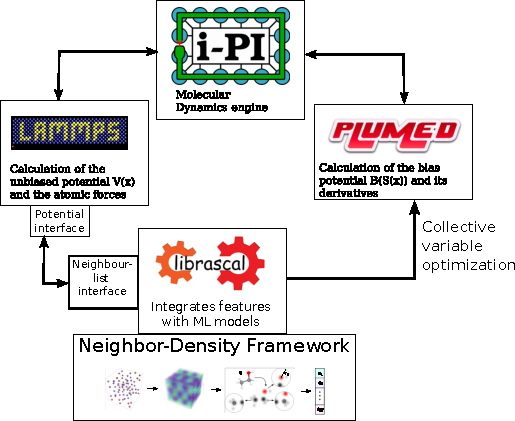
\includegraphics[width=\textwidth]{fig/ipi-librascal-plumed.pdf}
    \caption{A schematic showing the interwork of the software pieces to run metadynamic simulations to study interfacial effects of $BaTiO_3$.}
    \label{fig:ipi-librascal-plumed}
\end{figure}

This allowed obtain results...

\section{Modularity in MLIP}
There are several things we learn from technical analysis details that prevent a modular design as present it exists for traditional machine learning algorithms.
Narative:
An essential prevention for modularity is that the computation of the kernel requires a sparse data format hash mappable due to the species polynomial growth
Secondly, most ML packages do not support gradients in their methodology.
A recent develompent.

%\subsection{MLIP interface}

\section{Serialization of ML models}
In last decade, the rapid development of machine learning models has resulted in numerous interfaces for LAMMPS\cite{TODO}.
While the model accuracy is a good indicator for the usability of a model, it is still not reliable enough to be a guarantee that the model will work for MD software as undersampling of the phase space can always be an issue for any kind of model.
One is therefore forced to retrain the model for a dataset covering a larger part of the phase pace or switch to a more accurate model during the analysis of an experiment.
As all ML models show different trade-offs between accuracy, evaluation time, trainings cost and hyperparameter optimization the set of suitable models depend on the system of interest, the dataset size and given computational resources.
As the dataset size changes over the course of analysis different models become more suitable candidates and thus a different model is more suitable.
%It has been shown that linear models can be competetive in high data regime. %TODO verify that
The current software infrastructure of ML models for MD software causes a lof of friction when changing the model type as a new package needs installed and a new workflow pipeline has to be constructed.
Similar problems exists in industry where models trained with different ML packages need to be shipped to devices with different hardware architectures and different software stacks making it hard to reliably provide the same version of the package on the device.
Furthermore one would like to apply the same model in different

%Since the majority of ML models are constructed in higher-level languages, most MD engines are written in a low-level language for performance reasons.
%It is thus needed to export models to a standardized formate that allows to execute models in the low-level languaes
%Low-level language for efficiency, scripting-like for flexibility

Therefore serialization is essential. 
%to export models to one software from memory to disk for reproducibility and hardware independency (e.g. JSON).

\subsection{ONNX}

Explain how ONNX works and limitations of gradients

Heteregoneous hardware optimizer: OneAPI, Kokkos

\subsection{OpenKIM}

While OpenKIM addresses the problem of reimplementing the same interface for every MD engine.
It does not address the problem in language flexibility.

\subsection{TorchScript}
Allows gradients, limits one to torch

%\section{Foreign-Function interface [optional]}
%Low-level language for efficiency, scripting-like for flexibility
%Libraries that https://www.swig.org/compat.html
%Check out \url{https://docs.rs/rust_swig/latest/rust_swig/#enums}
%However these are not working with TorchScript, also Julia is missing that is becoming essential for scientific softwared development

%\section{Machine learning ecosystems}
%
%\subsection{Hardware kernels}
%\subsection{scikit-learn - close-form inspired infrastructure}
%- transformers, models
%- fit function needs to be specified that optimizes one object
%- concatenation of models through Pipelines allows parameter optimization over different modules however it is every rigid (sample dimension cannot change over the pipelines)
%\subsection{torch - autograd inspired infrastructure}
%Dataloader:
%- concatenation of indicies
%- caching
%Optimizer:
%- concatenation of indicies
%- caching
%While torch summarizes all existing optimizers under one library, Jax approaches this issue with modularity\cite{jaxopt_implicit_diff}
%\subsection{Standardization array-APIs}
%mention Array-API
%https://data-apis.org/array-api/latest/
